\documentclass{article}
\usepackage[utf8]{inputenc}
\usepackage[english]{babel}
\usepackage{graphicx}
\usepackage{amsmath}
\graphicspath{ {images/} }

\begin{document}
% Title page
\begin{titlepage}
    \vspace*{\stretch{1.0}}
    \begin{center}
        \Large{Udacity Machine Learning Nanodegree Capstone}\\
        \LARGE\textbf{Quora Duplicate Question Detection}\\
        \vspace{1cm}
        \large\textit{Raahul Seshadri}\\
        \normalsize{April, 2017}
    \end{center}
    \vspace*{\stretch{2.0}}
\end{titlepage}

% Table of contents
\tableofcontents
\newpage

% Begin sections
\section{Definition}

\subsection{Project Overview}
Websites like Quora\footnote{https://www.quora.com}, StackExchange\footnote{https://stackexchange.com} network (includes the popular programming website StackOverflow\footnote{https://stackoverflow.com}) allow the users to post questions, and the entire community can answer those questions. Ideally, every unique question should be present just once in the system, so that every answer to those questions are present at once place.

However, users are prone to posting duplicate questions, because not all of them check if the question they're asking has already been asked by someone else. This necessitates having an automated duplicate question checker that can check if a question is a duplicate. Whenever the user tries to post a new question, the system can suggest an existing one for perusal.

This project was inspired by Quora's Kaggle challenge\footnote{https://www.kaggle.com/c/quora-question-pairs}. A dataset of question pairs, manually tagged as duplicate or not by human reviewers, has been provided\footnote{https://www.kaggle.com/c/quora-question-pairs} by Quora to train on.

\textbf{For the purpose of this project, the inputs are strictly assumed to be in English.}

\subsection{Problem Statement}

The problem can be stated as follows:

\begin{center}
\textbf{Given a pair of question texts, detect if they are duplicate or not.}
\end{center}
For example, given the following two questions:

\begin{center}
\textit{Q1: What is the average salary in India?}\\
\textit{Q2: What is the average salary in the United States?}
\end{center}
The system could flag them as either duplicates or not-duplicates. The steps to achieving our duplicate detector are as follows:

\begin{enumerate}
\item{Download and pre-process the Quora training dataset}
\item{Split the Quora training dataset into 90\% training and 10\% test set.}
\item{In the 90\% training set, further 10\% will be used as a validation set.}
\item{Extract usable features from the dataset.}
\item{Train a binary classifier to differentiate between duplicates/non-duplicates.}
\item{Provide a command-line interface so that users can check for duplicates from Quora's test set, or provide his own questions.}
\end{enumerate}

\subsection{Metrics}

Being a binary classification problem, the metric is going to be accuracy:

$$\text{accuracy} = \frac{\text{true positives} + \text{true negatives}}{\text{total samples}}$$
This accuracy will be measured on the test set (10\% of the total dataset).

\begin{enumerate}
\item{\textbf{False negatives}, where a duplicate pair is not detected as such, will lead to degraded user experiences. However, it is also rather harmless, since no information is lost. There is still an opportunity to manually flag them as duplicates, or build such a feature on the platform that is using the duplicate detector.}
\item{\textbf{False positives}, where a question pair that's not a duplicate, but is marked as such, is more dangerous. It can lead to very degraded user experience, since it directly hinders the user trying to perform an action. It is better for the system to err on the side of false negatives than false positives.}
\end{enumerate}

\newpage
\section{Analysis}

\subsection{Data Exploration}

Below is the head (first 20 entries) of the Quora dataset:

\noindent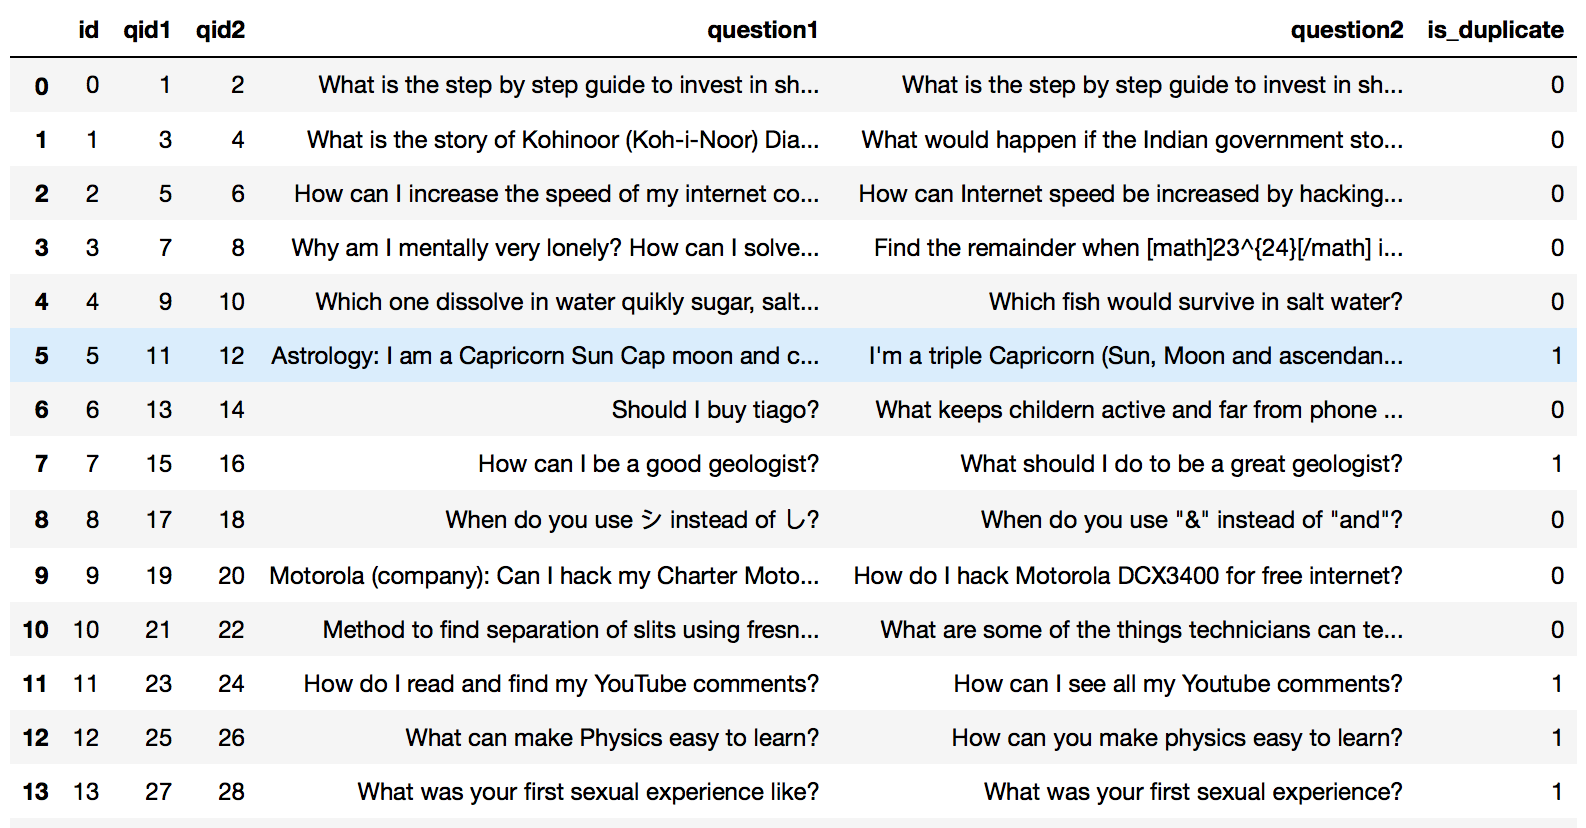
\includegraphics[width=\textwidth]{data_head}
The columns correspond to the following features:

\begin{enumerate}
\item{\textbf{id:} ID to identify the question pair uniquely}
\item{\textbf{qid1:} ID of the first question in the question pair}
\item{\textbf{qid2:} ID of the second question in the question pair}
\item{\textbf{question1:} Text of the first question in the question pair}
\item{\textbf{question2:} Text of the second question in the question pair}
\item{\textbf{is\_duplicate:} Quora reviewer's decision on whether the question pair is duplicate (1) or not (0)}
\end{enumerate}

\subsubsection{Why do we have question IDs for each pair?}
There are two columns of interest, ``qid1'' and ``qid2'' that are of interest. The algorithm that we're going to design will only tell us if a given pair of question is a duplicate. However, given a question, we'd also like to find out all the duplicates of it in the system.

For example, if question ``1'' is a duplicate of question ``2'', and question ``2'' is a duplicate of ``3'', then a system should also know that ``1'' and ``3'' are duplicates. Data structures like ``union find'' allow us to do that. However, this is not in scope of the algorithm that we'll design, but the responsibility of the higher system that will use this duplicate detector.

Which is why the question IDs won't be used as a feature for the duplicate detector, but is still important for the system using the duplicate detector.

\subsubsection{Summary statistics}

Below are some basic summary statistics:

\begin{enumerate}
\item{\textbf{Total entries:} 4,04,290}
\item{\textbf{Total positive entries:} 1,49,263}
\item{\textbf{Total negative entries:} 2,55,027}
\item{\textbf{Percent positive entries:} 36.91\%}
\item{\textbf{Percent negative entries:} 63.08\%}
\end{enumerate}

We have a sample with more negative than positive examples.

\subsection{Exploratory Visualization}

\subsubsection{Summary visualization}

Let's look at the class distribution (duplicate or not). This is the same from our summary statistics.

\noindent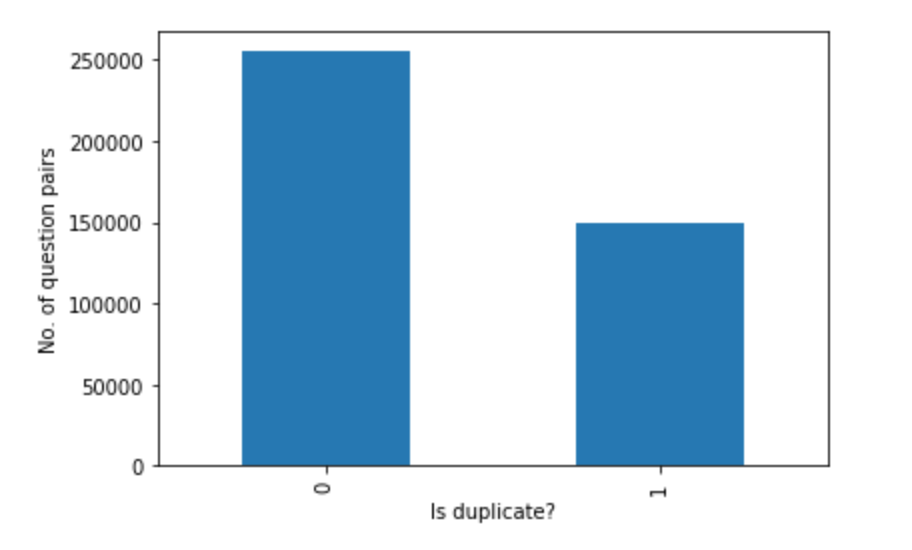
\includegraphics[width=\textwidth]{category_plot}

\subsubsection{Word count differences}

Let's look at if word count has any bearing on whether a question is marked as duplicate or not, or can we discern any important facts/patterns.

\noindent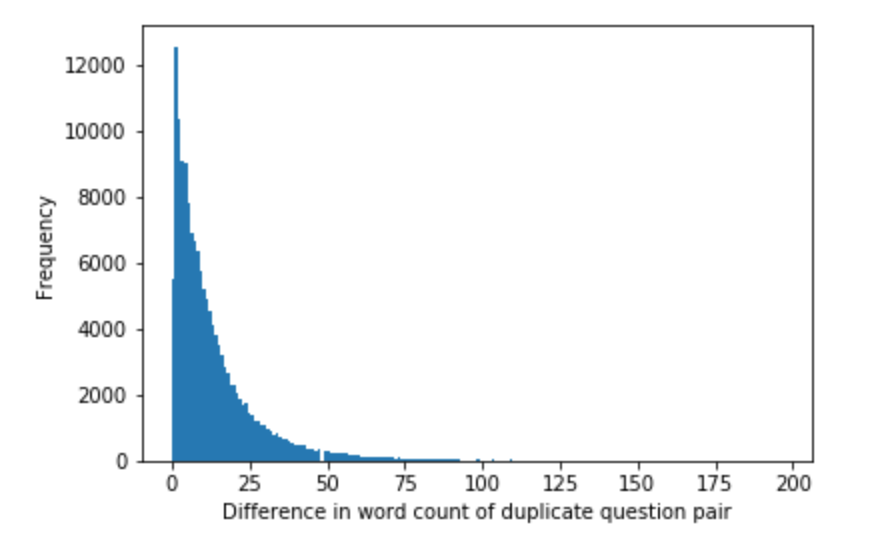
\includegraphics[width=\textwidth]{diff_wordcount_duplicate}
\noindent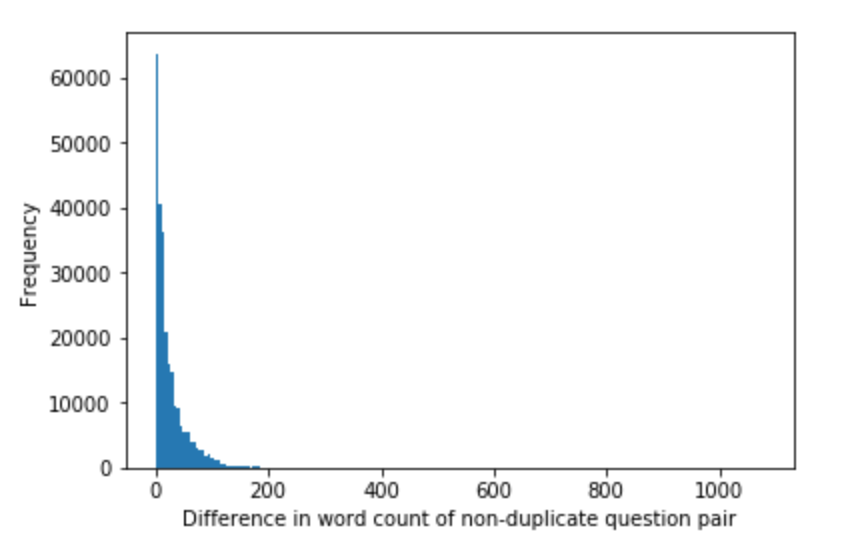
\includegraphics[width=\textwidth]{diff_wordcount_non_duplicate}

\begin{enumerate}
\item{For duplicates, the word count difference tapers smoothly}
\item{For non-duplicates, there is a sharp decrease in the 2nd bin}
\item{There are question pairs that have word count difference 75 and above, and are still duplicates. So simple bag of words model will not work. \textit{This is the most important conclusion.}}
\end{enumerate}

\subsubsection{Jaccard index}

To explore a baseline model, let's look at the bag-of-words similarity of duplicate and non-duplicate question pairs using the Jaccard Index\footnote{https://en.wikipedia.org/wiki/Jaccard\_index}. The relevant formula is:

$$
J(A,B) = \frac{A \cap B}{A \cup B}
$$

In our case, A and B refer to individual words in the question pairs. So, the formula basically is:

$$
J(A,B) = \frac{\text{No. of common words in question1 and question2}}{\text{No. of unique words in question1 and question2 combined}}
$$

Let's look at the Jaccard similarity of duplicate and non-duplicate question pairs separately.

\noindent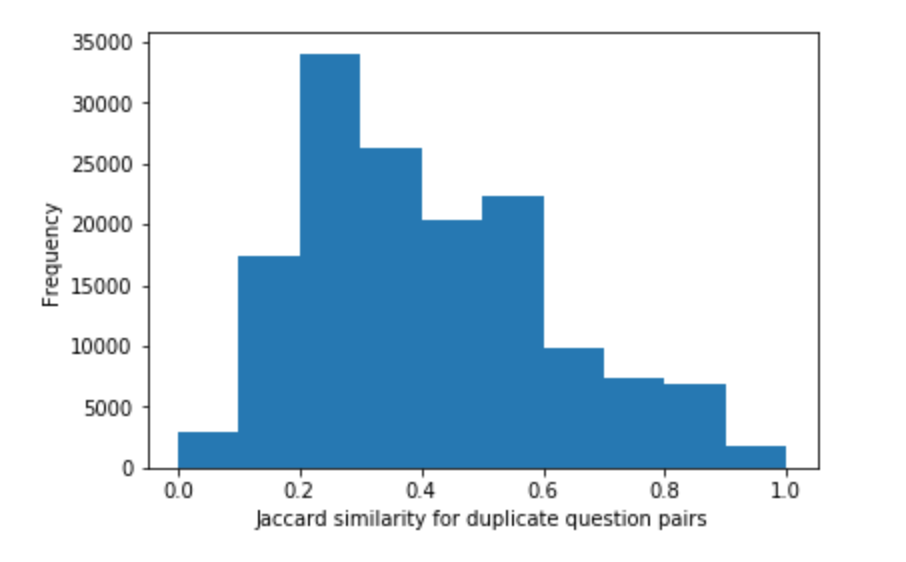
\includegraphics[width=\textwidth]{jaccard_duplicate}
\noindent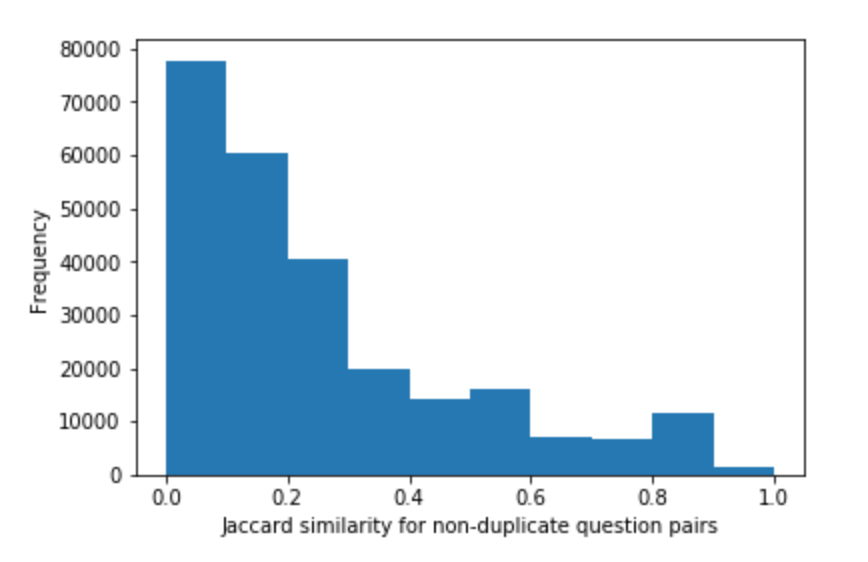
\includegraphics[width=\textwidth]{jaccard_non_duplicate}

\begin{enumerate}
\item{For duplicates, Jaccard similarity is like a gamma distribution. Jaccard is bad at predicting a pair is a duplicate.}
\item{For non-duplicates, the distribution is again gamma but with a right skew. So Jaccard positively gives low scores for most of the non-duplicates.}
\end{enumerate}

We had previously concluded from the word counts that bag-of-words similarity will not be a good method of differentiating between duplicates and non-duplicates, and the two graphs above confirm the fact.

\subsection{Algorithms \& Techniques}

\subsubsection{Feature extraction}

The inputs to our algorithm are two variable length strings. In NLP (Natural Language Processing), there are two primary ways of extracting features from text, after the input has been word-tokenized, that is being split into individual words:
\\\\
\noindent\textbf{Bag of words:}\\
Here, every word is assigned a unique number. The input to any ML algorithm then becomes a one-hot encoded array of numbers that correspond to these words.

For example, if the input corpus has two words: ``hello'' and ``world''. And we assign 0 to ``hello'' and 1 to ``world''. Then, the word ``hello'' would be represented as $[1\ 0]$ while ``world'' would be represented as $[0\ 1]$. (one hot encoded).

The number of features become equal to the number of unique words in the corpus (training set).
\\\\
\noindent\textbf{Word vectors:}\\
The problem with one hot encoding is that we come up with very large feature vectors, since they're one hot encoded. This does not scale to large corpora.

Instead of a sparse array, word vectors convert input words into a fixed-length vector. A common vector size is 300. Thus, every word in the input corpus gets converted into a dense feature vector of length, say, 300, regardless of how many words there are in the corpus.

As opposed to bag of words, word vectors have to be trained on a corpus, before they can be used to extract features from different corpora. Thankfully, there are a lot of pre-trained models for word vectors available.

Two popular algorithms to generate them are Word2Vec\footnote{https://en.wikipedia.org/wiki/Word2vec} and GloVe\footnote{https://nlp.stanford.edu/projects/glove/}. spaCy\footnote{https://spacy.io} comes with a GloVe model\footnote{https://spacy.io/docs/usage/word-vectors-similarities} of 300-dimensional vectors trained on the Common Crawl corpus. This is the Python library that we will use to do all our processing.

Naturally, I'll be using the word vectors approach, since it also allows me to train for words that don't appear in the Quora training corpus, but a similar word does.

\subsubsection{Pooling}

Given a pair of questions, the questions themselves can be of different sizes. If we get word vectors for each word in the question, then we get a matrix of size $m \times 300$, where we're assuming that $300$ is the word vector size and $m$ is the number of words in the question.

However, for a pair, $m$ could be different. Thus, we need a way to normalize this. There are two ways\footnote{https://explosion.ai/blog/quora-deep-text-pair-classification\#example-neural-network}:

\begin{enumerate}
\item{\textbf{Max pooling:} Take the maximum of each column in the $m \times 300$ matrix to get a $1 \times 300$ matrix.}
\item{\textbf{Mean pooling:} Take the mean of each column in the $m \times 300$ matrix to get a $1 \times 300$ matrix.}
\end{enumerate}

Max pooling is reported to perform better\footnote{https://explosion.ai/blog/quora-deep-text-pair-classification\#results}. However, I've decided to concatenate mean and max pooling to get a matrix $1 \times 600$ in dimension. Thus, every question is converted into 600-dimensional vector.

\subsubsection{Neural Networks}

We will be using Neural Networks to create our model. Neural Networks, especially deep ones, have lately become popular in the field of NLP.\footnote{http://colah.github.io/posts/2014-07-NLP-RNNs-Representations} \footnote{https://www.quora.com/How-are-neural-networks-used-in-Natural-Language-Processing} \footnote{https://nlp.stanford.edu/projects/DeepLearningInNaturalLanguageProcessing.shtml}

A neural network learns to model functions, just like supervised algorithms. However, the deeper the neural network (deeper meaning more number of layers), the more complex characteristics it can detect in the input.

A downside to neural networks is that it is incredibly difficult to correctly design them. The network structure itself has many possibilities, and then we also have a number of hyperparameters like epochs, depending on the optimizer being used. They also take a long time to train.

\subsubsection{Improving Neural Network Accuracy}

There are several techniques in neural networks to improve the accuracy of the network, or to reduce overfitting.
\\\\
\textbf{Dropout:}\\
Here, random units inside of the network are switched off in every epoch. Thus, the network is forced to learn redundant representations of the input. This, in totality, avoids overfitting. Dropout only happens during training, and is switched off when running the model in production.\footnote{https://www.quora.com/How-does-the-dropout-method-work-in-deep-learning} \footnote{https://www.cs.toronto.edu/~hinton/absps/JMLRdropout.pdf}

Due to the low amount of training data that we have, I'm not using dropouts in my network.
\\\\
\textbf{Batch Normalization:}\\
A Batch Normalization layer shifts the inputs from the previous layer to have zero-mean and unit-variance. This prevents data flowing in the network to not become too big or too small. It is said to result in higher accuracy and faster learning (convergence).\footnote{https://www.quora.com/Why-does-batch-normalization-help} To try this out, I trained variants of my network with Batch Normalization on and off.

\subsection{Benchmark}

In the field of Information Retrieval, there is a problem called Near Duplicate Detection.\footnote{https://nlp.stanford.edu/IR-book/html/htmledition/near-duplicates-and-shingling-1.html} Jaccard Similarity of bag-of-words ($k=1$ shinglings) is one way of finding near duplicates.\footnote{http://stackoverflow.com/questions/23053688/how-to-detect-duplicates-among-text-documents-and-return-the-duplicates-similar}

Since we split Quora dataset into 10\% test set, this benchmark model would be run on the test set. This baseline model gives an accuracy of $65.153\%$.


\section{Methodology}

\subsection{Data Pre-processing}

The Quora training dataset \textit{train.csv} is assumed to be in the same directory as the Jupyter Notebook.\footnote{Quora De-duplication.ipynb} The structure of the dataset is as in the exploration.

\subsubsection{Feature selection}

Out of all the columns in the dataset, we will use the following features:

\begin{enumerate}
\item{\textbf{question1:} Text of the first question in the pair}
\item{\textbf{question2:} Text of the second question in the pair}
\end{enumerate}

\noindent And the target variable:

\begin{enumerate}
\item{\textbf{is\_duplicate:} Whether the question pair is a duplicate or not. $1$ if it is, $0$ if it is not.}
\end{enumerate}

\subsubsection{Feature transformation}

A question from a question pair would go through the following transformations. For the examples below, we'll assume that the input text is ``This is a sentence'.'
\\\\
\textbf{Step 1: Tokenize text into words}\\
Using spaCy, we will convert a text like ``This is a sentence'' into words (tokens) like: ``This'' ``is'' ``a'' ``sentence''
\\\\
\textbf{Step 2: Get GloVe vectors for each word}\\
For every word, we get a GloVe vector of length $300$. Thus, we get a matrix of size $\textit{no. of tokens} \times 300$. In the case of our example sentence, it will be a matrix of size $4 \times 300$. This looks as shown below:\\\\

\begin{tabular}{|l|l|l|l|l|}
\hline
This     & 0 & 0 & ... & 0 \\ \hline
is       & 0 & 0 & ... & 0 \\ \hline
a        & 0 & 0 & ... & 0 \\ \hline
sentence & 0 & 0 & ... & 0 \\ \hline
\end{tabular}\\\\

\noindent\textbf{Step 3: Mean pooling}\\
The $n \times 300$ matrix is now converted into a $1 \times 300$ matrix by taking the mean of all the columns.\\

\noindent\textbf{Step 4: Max pooling}\\
The same $n \times 300$ matrix is converted again into a $1 \times 300$ matrix, but by taking the max from all the columns.\\

\noindent\textbf{Step 5: Concatenate mean and max. pooling}\\
The mean and max pool are concatenated into a matrix of size $1 \times 600$.

We repeat the above step for every question in every question pairs. This concludes our data pre-processing step. For our neural network, we will have two vectors of size $600$ as inputs.

\subsection{Implementation \& Refinement}

\subsubsection{Structure of the Neural Network}

\noindent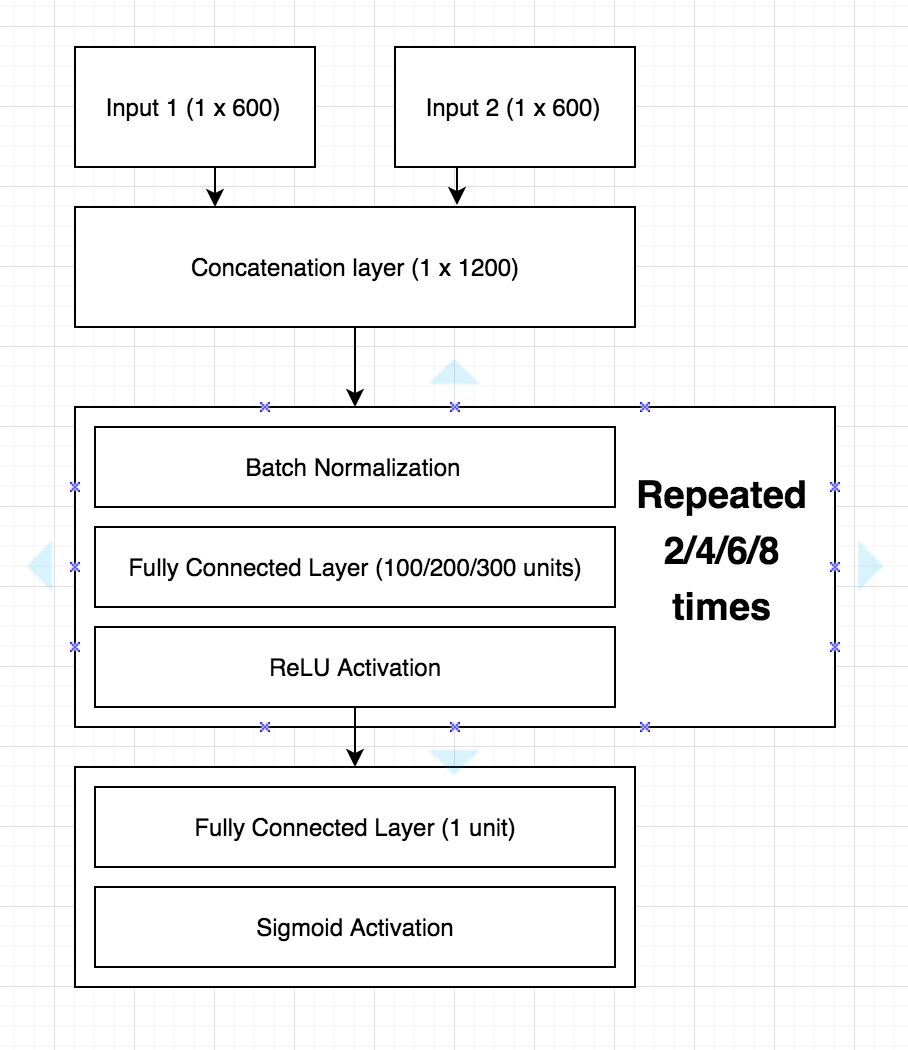
\includegraphics[width=\textwidth]{neural_network}

The following are the characteristics of this network:

\begin{enumerate}
\item{There are two inputs to the network, which are the $1 \times 600$ feature for each of the question in a pair.}
\item{These inputs are concatenated into one layer of size $1 \times 1200$.}
\item{A learning unit consists of a dense layer with ReLU activation, preceded by batch normalization.}
\item{The final layer is a dense layer with 1 neuron and sigmoid activation. This reflects the probability that a question pair is a duplicate.}
\end{enumerate}

To find the right network topology that will improve accuracy, we will try a couple of combinations.

\begin{enumerate}
\item{Number of training units: 2, 4, 6, 8}
\item{Number of neurons in the dense layer: 100, 200, 300}
\item{Batch normalization: True, False}
\end{enumerate}

This gives rise to 24 combinations. We will train the neural network on all of those topologies. The number of epochs is set to 25, because that is the maximum I have the resources to train 24 neural networks on. However, the training and validation accuracy of each epoch is put in a log, so that we can always check later for patterns of overfitting.

\subsubsection{Loss \& Optimization}

Binary crossentropy is used as a loss metric, since it's a binary classification problem. I used the adam optimizer, so as to avoid having to tune a lot of hyperparameters related to the optimizer by hand.

\subsubsection{Code Implementation}

To implement this neural network, we will use Keras\footnote{https://keras.io/}, which is a library that sits on top of Theano\footnote{http://deeplearning.net/software/theano/} and TensorFlow\footnote{https://tensorflow.org}. We will be using the Theano backend.

A neural network is created for all 24 combinations. A single function automatically generates a neural network given a combination. The naming convention for each model is ``\textit{no\_neurons\_\_batch\_norm\_\_no\_units}''. Here's an example:

\begin{enumerate}
\item{\textbf{No. of training units:} 2}
\item{\textbf{No. of neurons in dense layer:} 200}
\item{\textbf{Batch normalization:} True}
\end{enumerate}

In this case, the model will be named ``200\_True\_2''. The model will be saved to disk as ``200\_True\_2.h5'', and the log of training would be saved as ``200\_True\_2.h5.log''.

\subsubsection{Final performance}

The model that performed the best, with test accuracy of \textbf{82.783\%} has the following characteristics:

\begin{enumerate}
\item{Number of training units: 6}
\item{Number of neurons in the dense layer: 300}
\item{Batch normalization: True}
\end{enumerate}

The baseline solution had an accuracy of $65.153\%$ on the test set.

\subsubsection{Performance of intermediate models}

Let's look at how the 23 other neural network combinations performed.

\noindent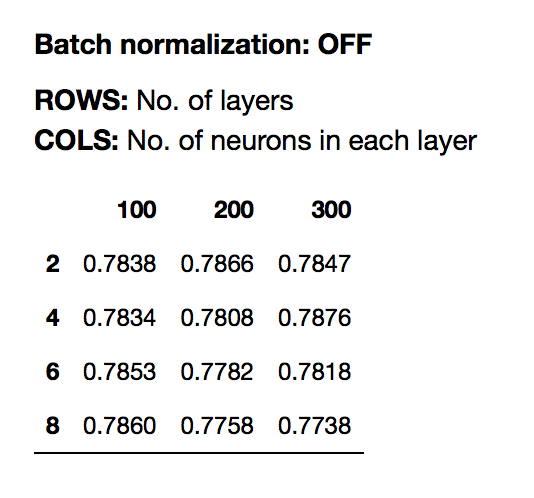
\includegraphics{perf_batch_off}\\
\noindent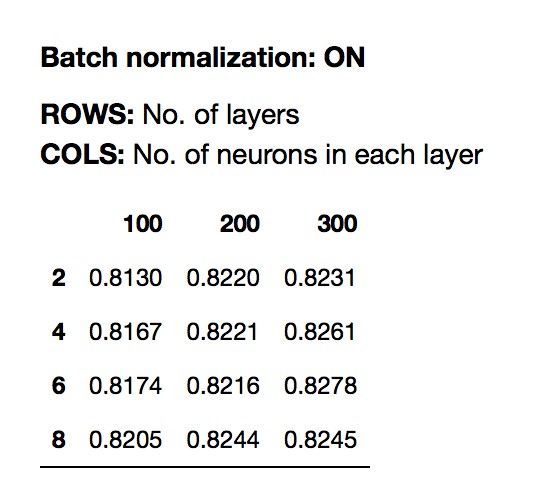
\includegraphics{perf_batch_on}

\newpage
The following observations can be made:

\begin{enumerate}
\item{The best performance with batch normalization OFF is \textbf{78.76\%}. With ON, it's \textbf{82.78\%}. There's a \textbf{4.02\%} improvement.}
\item{With batch normalization ON, the lowest test accuracy is \textbf{81.30\%}, and the highest test accuracy is \textbf{82.78\%}. Tuning of hyperparameters has lead to a \textbf{1.48\%} improvement in accuracy.}
\end{enumerate}

\section{Results}
\subsection{Model Evaluation, Validation, and Justification}

As mentioned previously, the model that performed best had the following characteristics, and a final test accuracy of \textbf{82.783\%}:

\begin{enumerate}
\item{Number of training units: 6}
\item{Number of neurons in the dense layer: 300}
\item{Batch normalization: True}
\end{enumerate}

The baseline solution had an accuracy of $65.153\%$ on the test set. Thus the neural network solution gave an improvement of \textbf{17.63\%} over the benchmark (that just naively compared bag of words and calculated the Jaccard index).

This final model had the following characteristics after 25 epochs (this data is obtained from ``300\_True\_6.h5.log''):

\begin{enumerate}
\item{Training accuracy: 91.300\%}
\item{Validation accuracy: 82.370\%}
\item{Test accuracy: 82.783\%}
\end{enumerate}

The training accuracy is higher than the validation/test accuracy, so the model is slightly over-fitting. The validation and test accuracy are close to each other, so the model does generalize well to unseen data. Given the accuracy score, we can say that the model has helped in solve the problem.

With more amount of training data, the accuracy can be improved further. With significantly more data, custom GloVe vectors can be trained instead of using a pre-trained model. This would ensure that the vectors reflect the nature of the data the duplicate detector will run on.

\section{Conclusion}

\subsection{Free-form Visualization}

The most important quality of interest is the ability to recognize entities in the question. I've come up with these questions myself as an experiment. For example, Quora reviewers consider the following to be NOT duplicate:
\\\\
\begin{tabular}{|l|l|}
\hline
Question 1 & What is the salary in the US? \\ \hline
Question 2 & What is the salary in Germany? \\ \hline
Human opinion & NOT DUPLICATE \\ \hline
Model's prediction & NOT DUPLICATE \\ \hline
\end{tabular}\\

The reason they're not duplicates is because they talk about two different countries, even though most of the keywords in the question are the same. Our model gets it right.

On the flipside, let's look at a pair of question that ask the same thing but in different words:
\\\\
\begin{tabular}{|l|l|}
\hline
Question 1 & How to learn programming? \\ \hline
Question 2 & How do I become good at programming? \\ \hline
Human opinion & DUPLICATE \\ \hline
Model's prediction & DUPLICATE \\ \hline
\end{tabular}\\
\\\\
\begin{tabular}{|l|l|}
\hline
Question 1 & Where do I go in Germany? \\ \hline
Question 2 & What are some good places to visit in Germany? \\ \hline
Human opinion & DUPLICATE \\ \hline
Model's prediction & DUPLICATE \\ \hline
\end{tabular}\\

Word vectors helps our model recognize the basic intents behind each question, and thus categorize similar words as one. Let's change the name of the country in the above example, and the question is no longer classified as duplicate. Thus the names of entities do matter a lot to the model.
\\\\
\begin{tabular}{|l|l|}
\hline
Question 1 & Where do I go in Germany? \\ \hline
Question 2 & What are some good places to visit in India? \\ \hline
Human opinion & NOT DUPLICATE \\ \hline
Model's prediction & NOT DUPLICATE \\ \hline
\end{tabular}\\

One problem of using pre-trained word vectors, is that they can flag entities as similar if they were commonly used together in the GloVe's training corpus. For example:
\\\\
\begin{tabular}{|l|l|}
\hline
Question 1 & Where do I go in Germany? \\ \hline
Question 2 & What are some good places to visit in France? \\ \hline
Human opinion & NOT DUPLICATE \\ \hline
Model's prediction & DUPLICATE \\ \hline
\end{tabular}\\

Here, the model incorrectly predicts them as duplicate. This is because France and Germany might have appeared in close contexts in the GloVe's training set, and GloVe thinks that both of those words have a strong connection, since they're both European countries.

This can be verified by computing the GloVe similarity between ``France'' and ``Germany'':

\noindent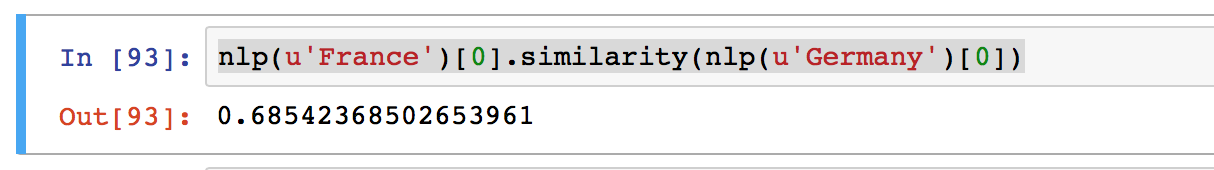
\includegraphics[width=\textwidth]{france_germany_similarity}

We can see a 68.5\% similarity between the two words, hence this explains the problem that we had with our last question pair. This type of false positives are very detrimental to the user experience.


\subsection{Reflection}

This entire project was about supervised learning. We had a target variable, and some form of primitive features. However, being a Natural Language Processing task, features had to be extracted from the text first.

\subsubsection{Feature extraction}

This aspect was the most important. Text is variable sized and arbitrary. Machine learning algorithms deal with numeric features. I explored the two commonly used option to go from text to numeric features, bag of words, and word vectors. The quality that made word vectors attractive was the fact that it could express similarity between words. So, not all the words in the dictionary needed to be present in the training corpus of the duplicate detector. The model could relate words it has never seen to words that it did see during training using word vectors.

The second point was getting to a fixed feature size from a variable length text. This is where max and mean pooling came in. Once every question has been converted into fixed length features, then it became ready for any ML algorithm to be applied.

\subsubsection{Training}

Due to the popularity and performance of deep neural networks in NLP, I decided to go with that route. However, the topology of the network has many possibilities. Although with experience, one can predict what kind of topology would be ideal, I decided to train on all combinations to find out what kind of improvement each factor brings in.

It took days to train all 24 network, but the results were worth the wait. Batch Normalization came out to be an important technique to improve accuracy.

\subsubsection{Interesting aspects of the problem}

Whether two questions are duplicate or not, does not depend on just the words that they use, but the intent of the question. As we observed in the Free-form Visualization section, questions can be framed differently, but can still be duplicates, and can be flagged as such. Entities become important, since changing them can change the duplicate detector's analysis.

I believe this final model does generalise well to these types of problem. The training corpus can be augmented, or we can get a different one depending on the domain, and the model will perform well for that domain. The only pre-requisite is that most of the words used in a domain should have GloVe vectors. For common scenarios, we can use a pre-trained one, or else we can train one on our own from the training corpus.

\subsection {Improvement}

\end{document}
